\documentclass[main_conf.tex]{subfiles}
\begin{document}

Las plantas de fabricación de mallas metálicas usan máquinas de
confección de hebras metálicas (MCHM) de diferentes grosores y
longitudes. Estas máquinas no suelen poseer una Interfaz
Humano-Máquina (Human-Machine Interface, HMI) para controlar
automáticamente sus procesos o modos de trabajo. Solo se 
cuenta con controles On/Off manual (ver Fig.
\ref{maquina_a_automatizar}.a). Por ende, se tiene una medición
de longitud de cada hebra manual, lenta y con grandes pérdidas.

Se implementa un sistema con el fin de reducir al máximo el
error de medición para así reducir la merma y reducir costos de
producción. Así mismo, este sistema será fabricado con materiales
de bajo costo y de fácil obtención en el mercado local.

\begin{figure}[t]
  \centering
  \begin{subfigure}[b]{0.5\textwidth}
    \centering
    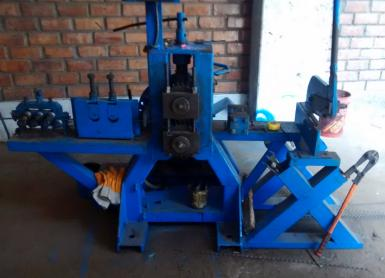
\includegraphics[width=2.5in]{../img/maquina/toda.jpg}
    \caption{Circuito de Potencia}
  \end{subfigure}

  \begin{subfigure}[b]{0.5\textwidth}
    \centering
    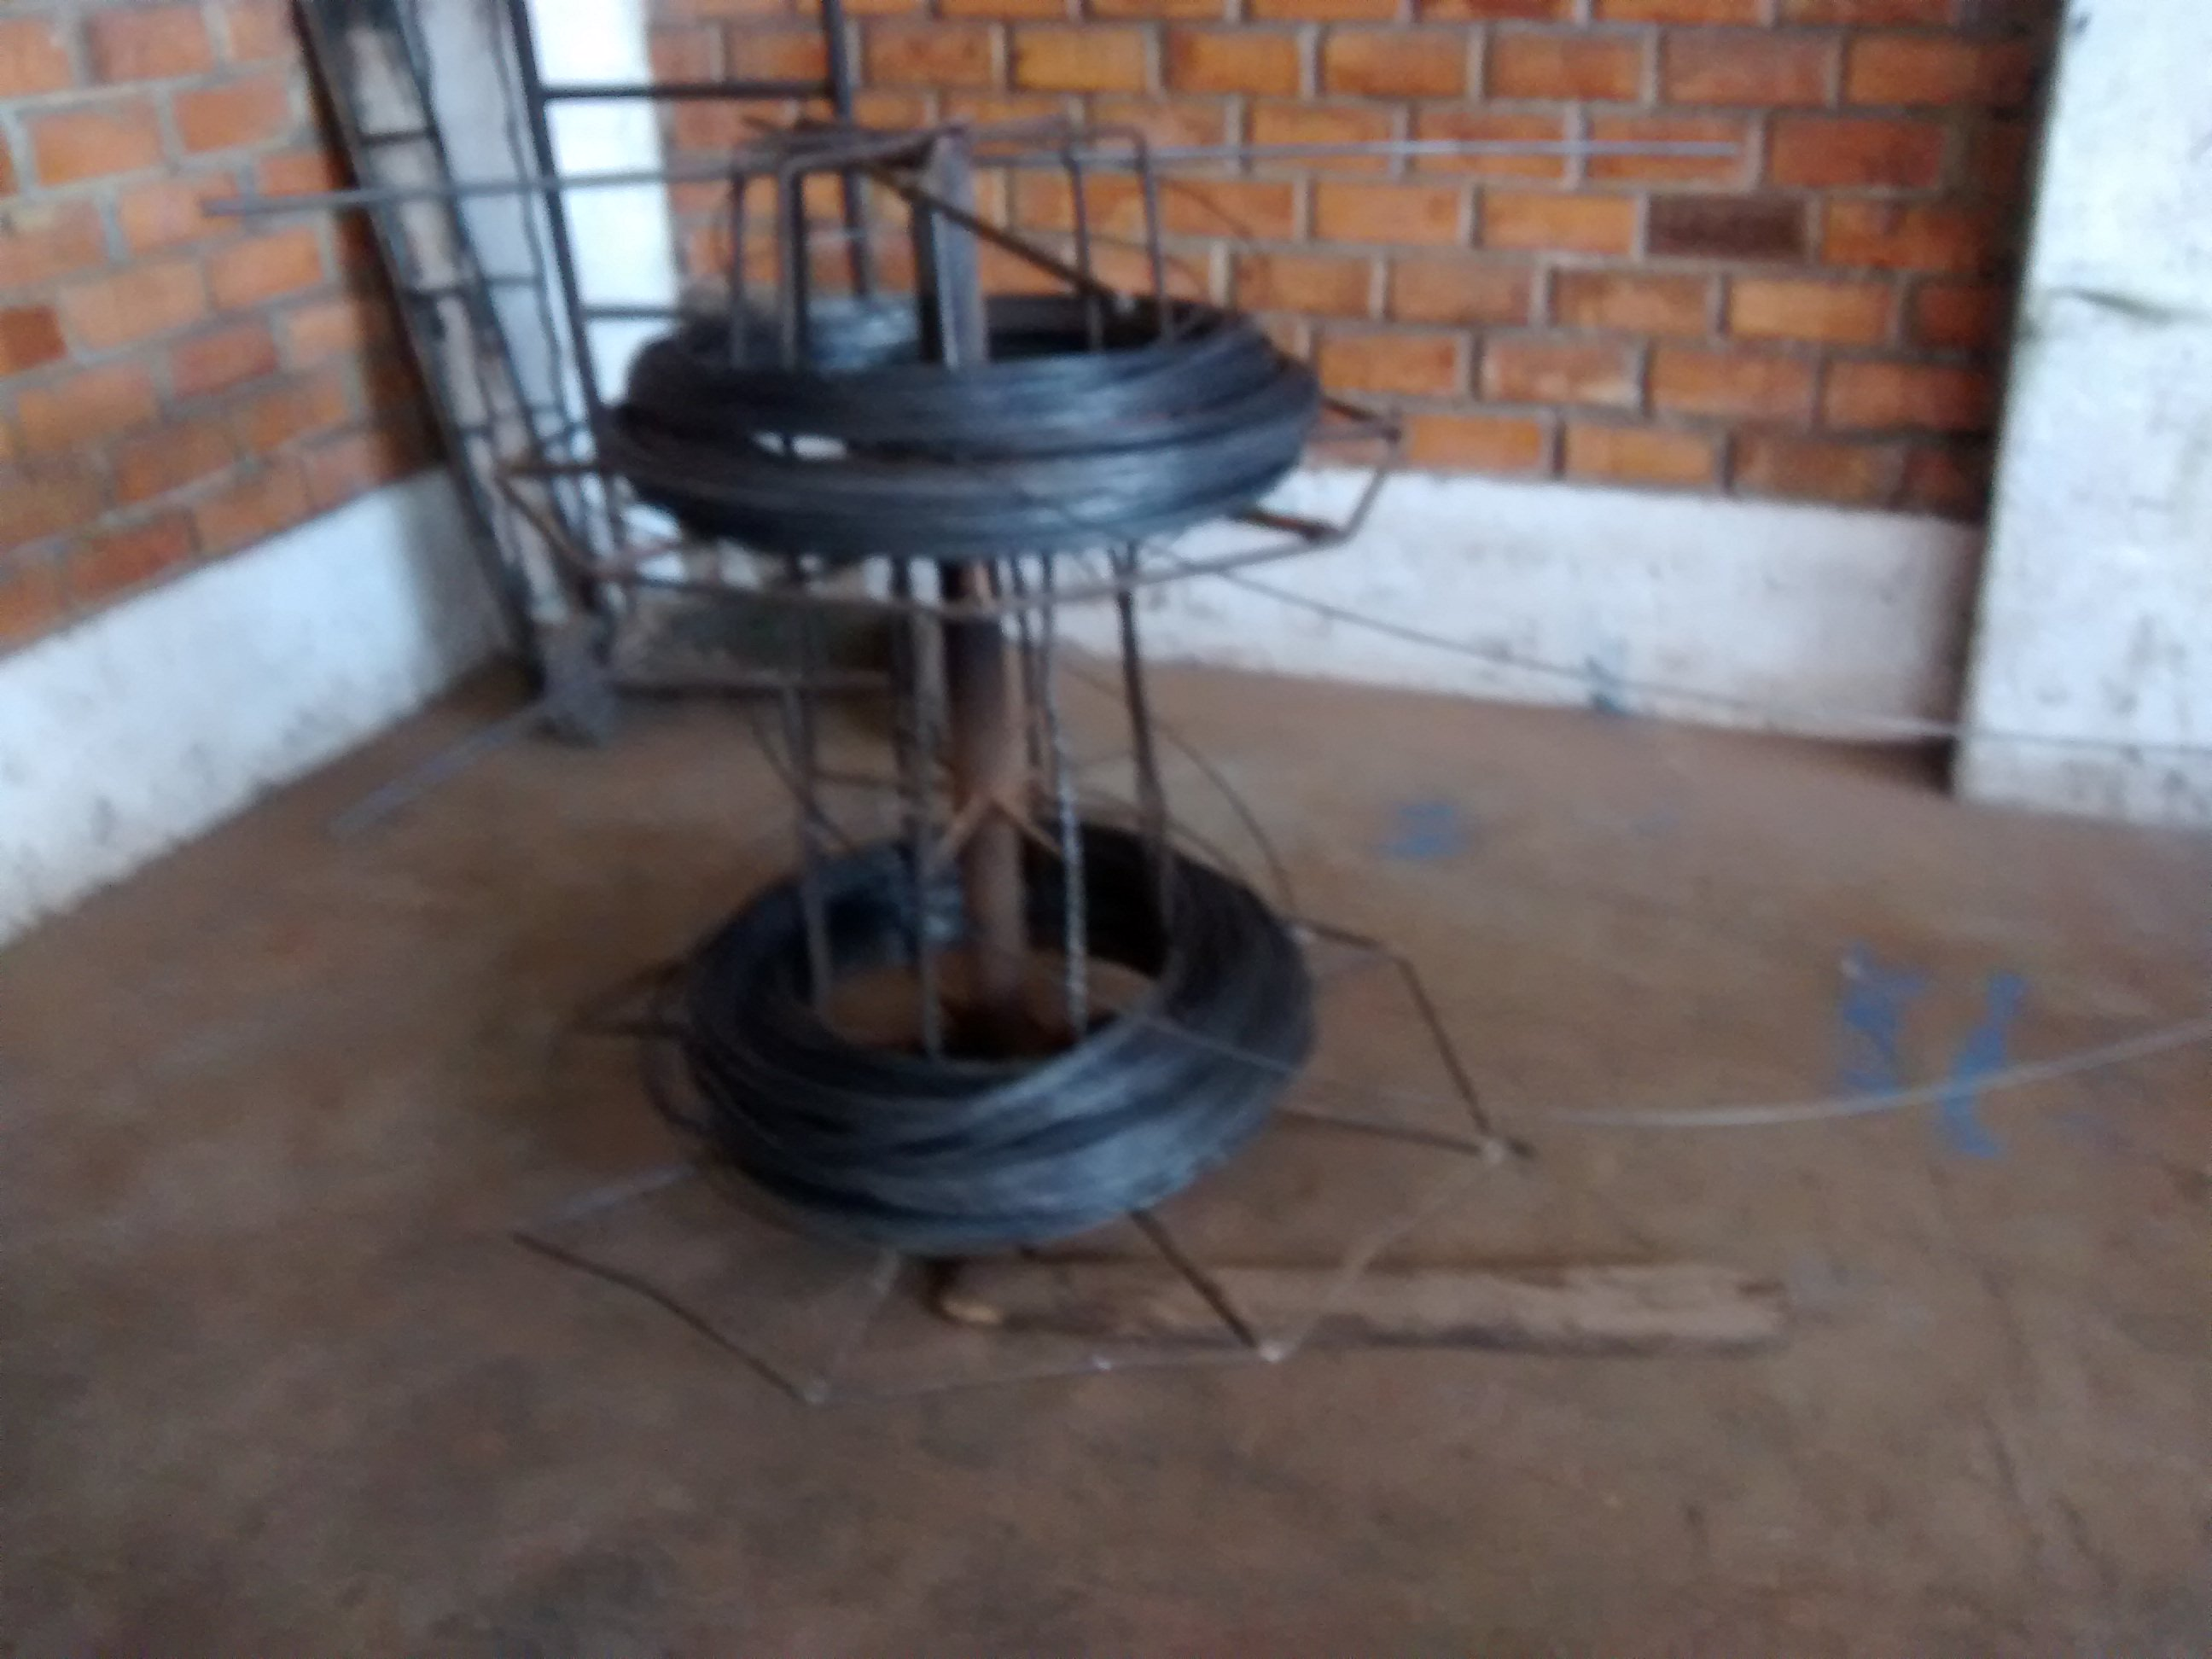
\includegraphics[width=2.5in]{../img/maquina/tambor.jpg}
    \caption{Tambor proveedor de HM}
  \end{subfigure}

  \caption{Rodillo con disco para encoder relativo}
  \label{maquina_a_automatizar}
\end{figure}


\begin{figure}[t]
  \centering
  \begin{subfigure}[b]{0.5\textwidth}
    \centering
    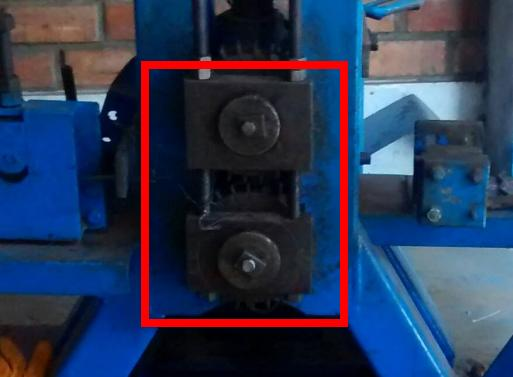
\includegraphics[width=2.5in]{../img/maquina/deformadores.jpg}
    \caption{Discos deformadores}
  \end{subfigure}

  \begin{subfigure}[b]{0.5\textwidth}
    \centering
    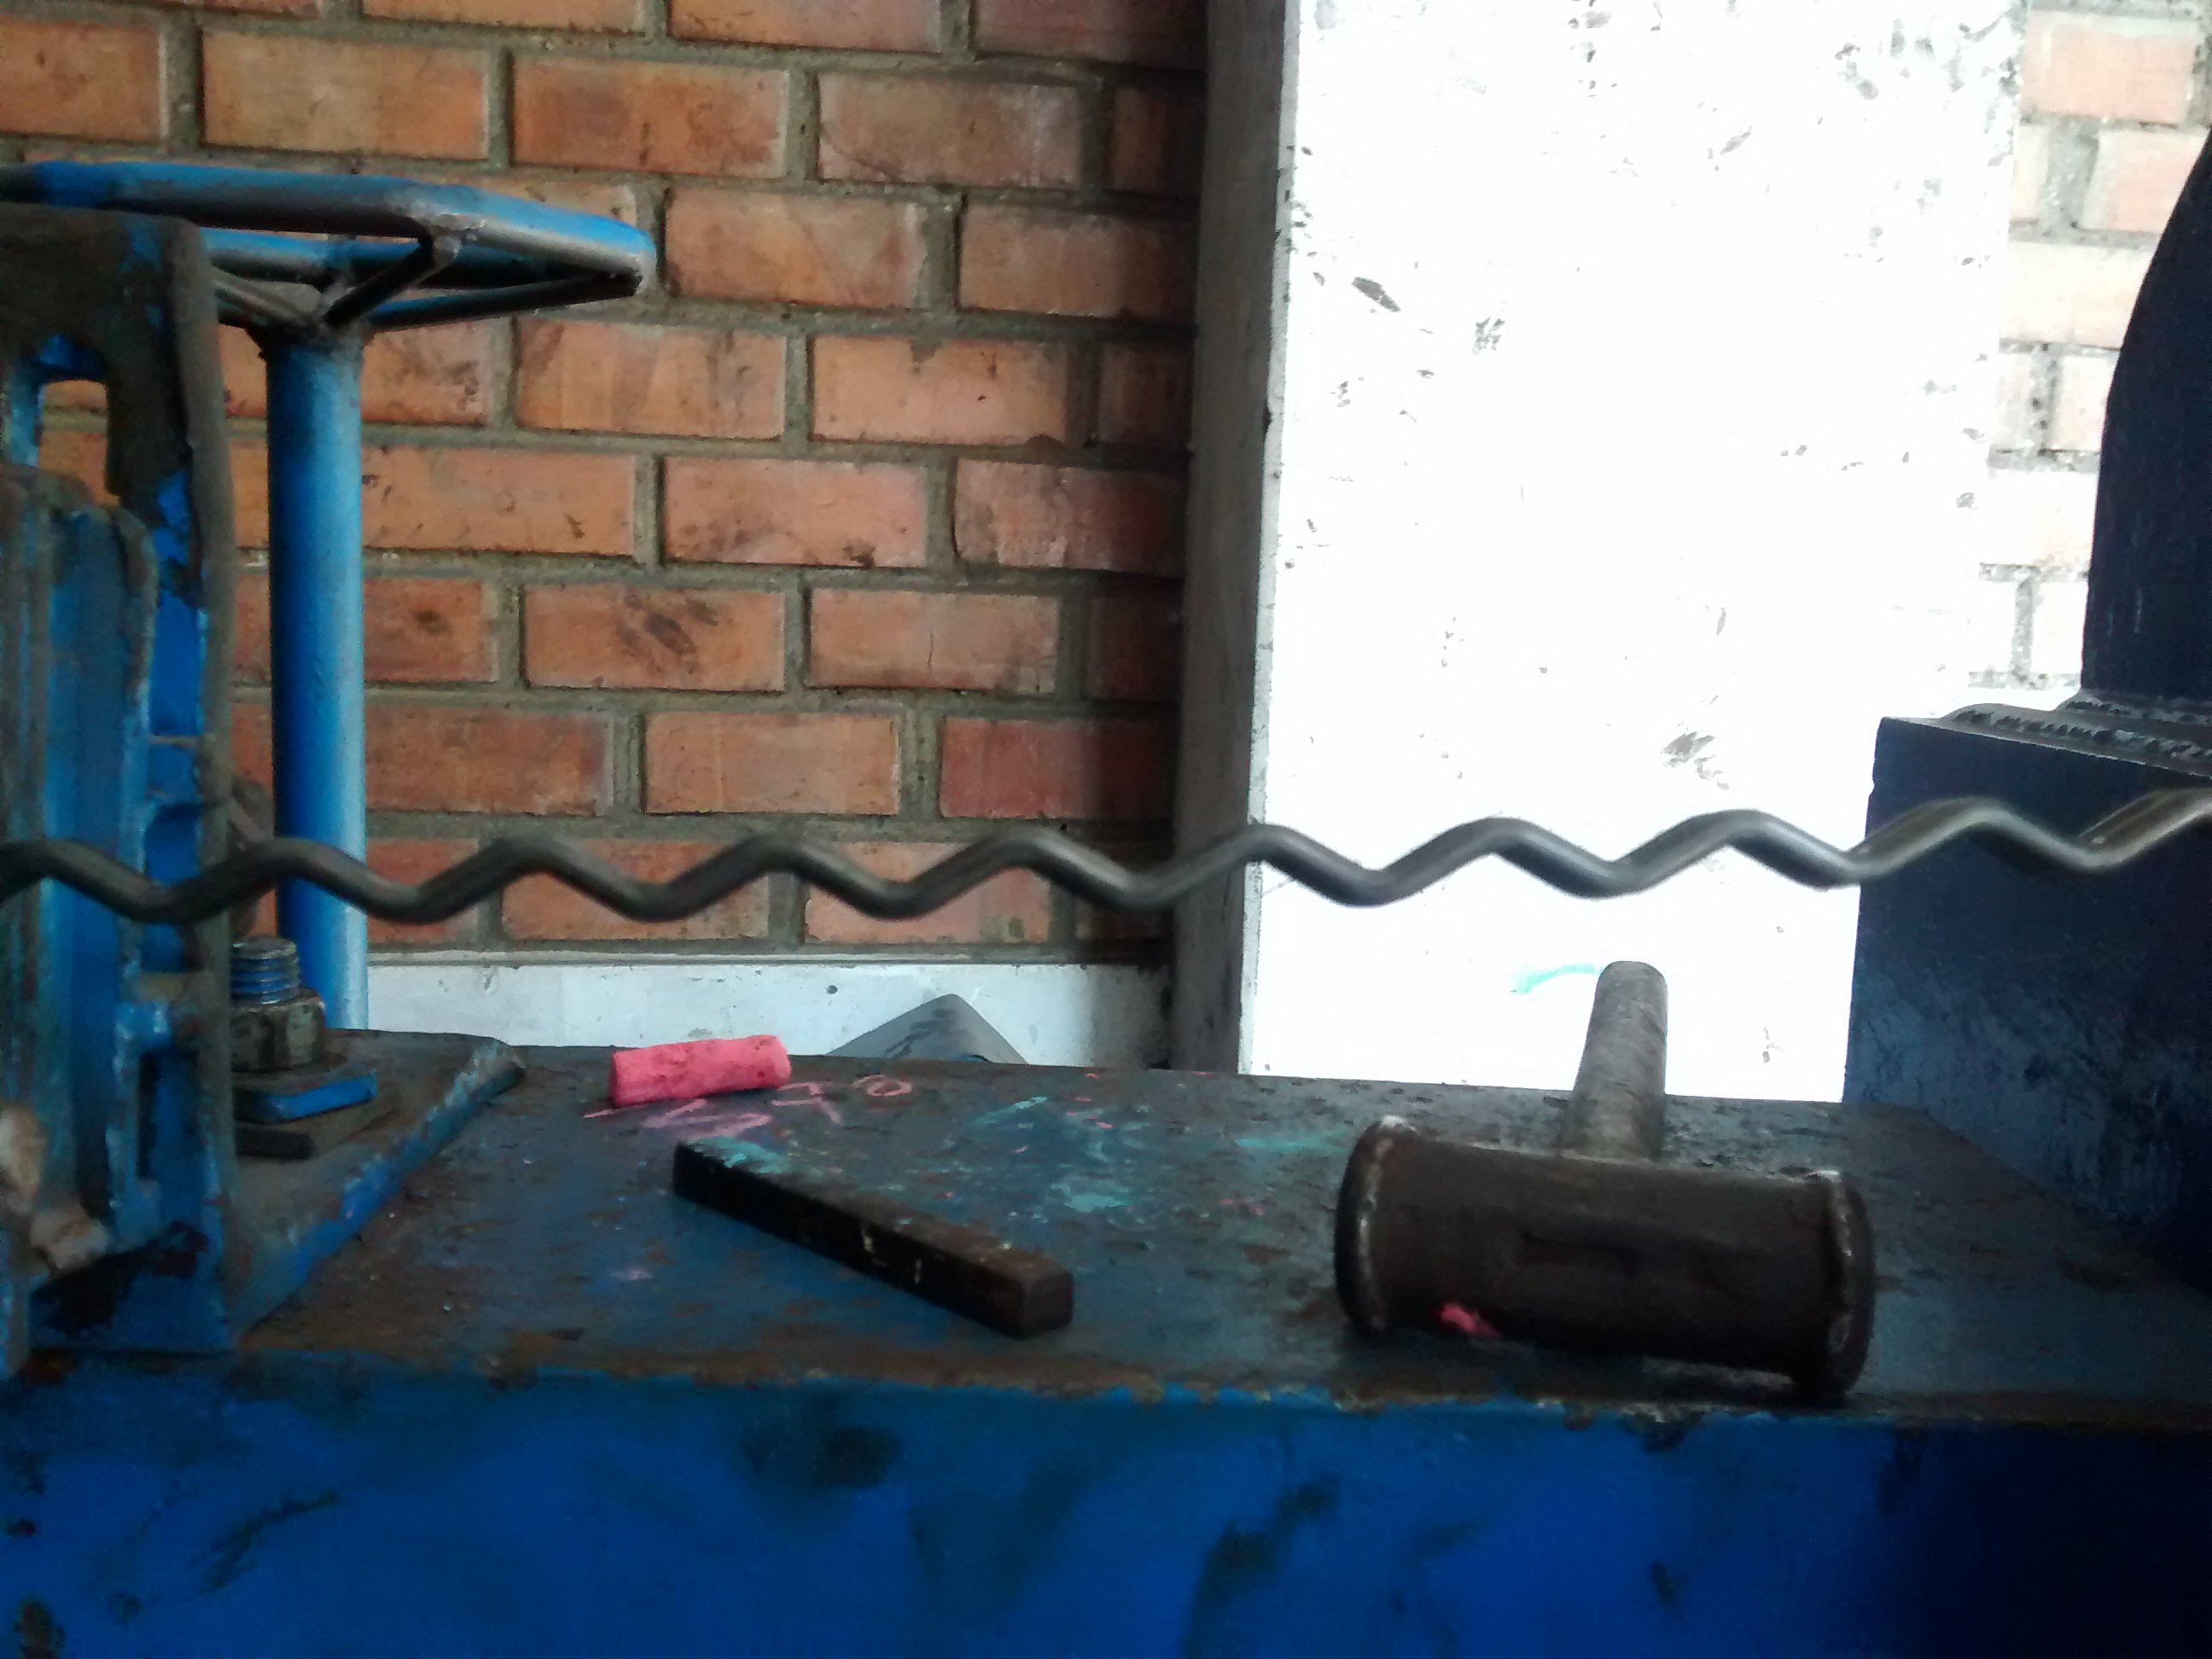
\includegraphics[width=2.5in]{../img/maquina/hebra.jpg}
    \caption{Hebra metálica tras deformación}
  \end{subfigure}

  \caption{Rueda dentada deformadora y hebra metálica}
  \label{maquina_a_automatizar}
\end{figure}


\subsection{Descripción de la máquina}
La MCHM es alimentada de un alambre de acero por un tambor
giratorio (TG) (ver Fig.\ref{maquina_a_automatizar}.b) y su función es
deformar este hilo para generar una hebra metálica (HM) mediante un
par de rueda dentadas del mismo tamaño y mismo número de dientes.
Existen 30 tamaños de estas ruedas (ver Fig.
\ref{maquina_a_automatizar}.c) que son empotradas en un par
de ejes que giran a la misma velocidad.

\subsection{Proceso manual a automatizar}
\label{sec:intro:proceso_manual}
El propósito de la máquina es proporcionar un número de $N$ HMs
de longitud $L$, por lo que el operador sigue el siguiente
procedimiento:

\begin{enumerate}
\label{enum:intro:descripcion_maquina}
\item Medir una longitud $L$ desde la cortadora
\item Marcar con tiza en el piso en el punto medido
\item Repetir $N$ veces:
  \begin{enumerate}
    \item Iniciar proceso hasta que la HM llegue a la marca
    \item Cortar la HM.
  \end{enumerate}    
\end{enumerate}

\subsection{Descripción de la solución}
Se construye una HMI para configurar o manipular los  diferentes
procesos o modos de operación de la MCHM y consta de un Arduino
Nano (AN) para controlar todo el proceso, una pantalla
y un teclado para configurar y monitorear los procesos,
mejor descritos en la sección \ref{sec:HMI}.

Se introduce dos rodillos que presionan la HM generada.
Producto de la fricción, los rodillos giran. Uno de estos es conectado a
un disco encoder con el cual se estima la longitud de la HM en proceso.

Se usa un Arduino Nano para adquirir las señales del encoder,

\end{document}
